Phần này trình bày các kết quả thu được từ nghiên cứu. Có thể sử dụng hình ảnh, bảng biểu minh họa kết quả, hỗ trợ cho phần bàn luận. Nhấn mạnh các đóng góp mới của nghiên cứu so với các nghiên cứu tương tự đã công bố.

Nếu cần thiết, có thể chia nội dung một phần của bài báo thành nhiều phần nhỏ. Khi này, có thể cung thông tin giới thiệu nội dung các phần nhỏ giữa tiêu đề của phần chính với tiêu đề của phần nhỏ đầu tiên. 

Tiêu đề các phần nhỏ (Tiêu đề cấp 2) thống nhất dùng chữ in nghiêng đậm, cỡ 11 như dưới đây.


\subsection{Chữ viết tắt}
\label{subsec:viet_tat}

Những thuật ngữ dài, được sử dụng nhiều lần có thể sử dụng chữ viết tắt. Thuật ngữ này cần được hiển thị đầy đủ ở lần đầu tiên xuất hiện trong bài viết, kèm theo ký hiệu viết tắt đặt trong ngoặc đơn. Ví dụ: "Các định hướng phát triển khoa học công nghệ (KHCN) đã đóng vai trò...".


\subsection{Các lưu ý định dạng và trình bày}
\label{subsec_Criterial}

\subsubsection{Đơn vị đo và số liệu}
Thống nhất dùng đơn vị đo theo hệ SI cho các số liệu trong bài báo. Định dạng in nghiêng cho ký hiệu các đại lượng tính toán. Số thập phân trình bày trong bài báo tiếng Việt để dấu ","; trong bài báo tiếng Anh để dấu "."


\subsubsection{Công thức toán}
Các công thức tính toán được đánh số thứ tự, đặt trong ngoặc đơn phía lề phải như minh họa bằng các công thức (1) và (2) dưới đây. Lưu ý là các ký hiệu hàm, biến được in nghiêng; ký hiệu ma trận, véc tơ được in đậm. 

\begin{equation}
	U_m(0,f) \geq u \geq \varphi + U_m(0,f)
\end{equation}
\begin{equation}
	U_m(0,f) - \alpha > c \varphi
\end{equation}

\subsubsection{Hình ảnh, bảng biểu}
Các hình ảnh (đồ thị, sơ đồ, ảnh chụp...), bảng biểu nhất thiết phải có số hiệu và tiêu đề. Số hiệu đánh theo thứ tự tăng dần của bài báo, ví dụ Hình 1, Hình 2; bảng 1, bảng 2... Số hiệu hình vẽ, bảng biểu phải được tham chiếu (giới thiệu, bình luận) trong văn bản. Khi biên tập, để phù hợp với format của trang báo, Tòa soạn có thể di chuyển vị trí của bảng biểu, hình vẽ lên đầu trang hoặc xuống cuối trang; Do đó, đề nghị tác giả không sử dụng cách giới thiệu tương tự như: "... được minh họa trong hình sau:", hay "Số liệu thống kê như trong bảng sau:". Cần tham chiếu đến số hiệu của hình, bảng, chẳng hạn như "... được minh họa trong Hình 1", hay "Số liệu thống kê như trong bảng 2".

Số liệu trong bảng phải chính xác, hình ảnh rõ nét. Độ rộng của bảng và hình vẽ bằng độ rộng của cột, hoặc của trang giấy theo khổ dọc. Nếu bảng và hình vẽ quá lớn có thể trình bày theo trang ngang (Landscape).

Cố gắng sắp xếp để hình ảnh, bảng biểu ở vị trí gần với nội dung văn bản có tham chiếu đến hình ảnh, bảng biểu.

Nếu một hình bao gồm nhiều hình nhỏ, ký hiệu các hình nhỏ bằng các chữ cái a), b), v.v... và giải thích nội dung các phần nhỏ ngay trong tiêu đề của hình.

\setlength{\intextsep}{0pt}
\renewcommand{\scalefigure}{0.8}
\noindent
\begin{figure}[h!]
	\centering
	\begin{subfigure}{.48\linewidth}
		\centering
		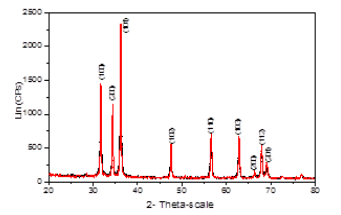
\includegraphics[scale=\scalefigure]{Pictures/pic2a.png}
		\caption{}
		\label{fig:giando_a}
	\end{subfigure}   
	\begin{subfigure}{.48\linewidth}
		\centering
		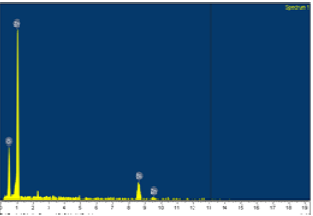
\includegraphics[scale=\scalefigure]{Pictures/pic2b.png}
		\caption{}
		\label{fig:giando_b}
	\end{subfigure}
	\caption{ (a) Giản đồ XRD của nano ZnO tổng hợp: (b) Phổ EDS của vật liệu nano ZnO }
	\label{fig:giando}
\end{figure}

Số hiệu và tiêu đề của hình để bên dưới hình. Số hiệu và tiêu đề của bảng nằm bên trên bảng. Chèn một dòng trắng vào bên trên hình và dưới tiêu đề của hình để ngăn cách với các phần văn bản phía trước và sau mỗi hình.

Hình~\ref{fig:giando} minh họa mẫu định dạng tiêu đề của một hình được chèn trong bài báo. Định dạng các thành phần của bảng biểu được minh họa như trong Bảng~\ref{tab:pt1}.

\setlength{\intextsep}{6pt}
\begin{table}[htbp]
	\centering
	\caption{Phân tích hàm lượng các nguyên tố trong lá chè (mg/kg)}
	\begin{tabular}{crrrrrrr}
		&       &       &       &       &       &       &  \\
		\midrule
		\textbf{Mẫu} & 
		\textbf{Mn} & 
		\textbf{Al} & 
		\textbf{Fe} & 
		\textbf{Zn} & 
		\textbf{Cu} & 
		\textbf{Ba} & 
		\textbf{Sr} \\
		\midrule
		MC1 & 741.92 & 260.22 & 61.88 & 31.85 & 13.64 & 13.04 & 14.95 \\
		MC2 & 1179.39 & 282.44 & 85.14 & 33.58 & 16.39 & 4.36  & 7.19 \\
		MC3 & 1239.37 & 273.67 & 86.6  & 34.69 & 15.23 & 11.97 & 8.4 \\
		MC4 & 923.03 & 281.94 & 81.48 & 31.28 & 15.58 & 6.1 & 7.61 \\
		MC5 & 918.55 & 201.7 & 67.41 & 39.79 & 14.62 & 7.04 & 9.14 \\
		MC6 & 613.33 & 189.2 & 65.76 & 27.67 & 14.55 & 12.12 & 10.56 \\
		\textbf{Trung bình} & \textbf{762.25} & \textbf{324} & \textbf{74.95} & \textbf{30.33} & \textbf{14.38} & \textbf{15.02} & \textbf{11.92} \\
	\end{tabular}%
	\label{tab:pt1}%
\end{table}%

\textbf{Lưu ý:} Các thành phần của bảng biểu phải ở dạng văn bản chỉnh sửa được, không để dưới dạng ảnh chụp màn hình. 

